\chapter{Beginning to Decode}

\section{Instruction Decode}

The next stage in the datapath is the iDecode stage.  The iDecode stage evaluates the binary instructions (an output of the iFetch stage) and determines what needs to be done.  There are many aspects to the iDecode stage, and some get fairly complex.  But today we will begin the process of decoding an instruction by decomposing the instructions into the key parts of R-Type and D-Type instructions:
\begin{enumerate}
	\item opcode
	\item address (used only in D-Type instructions)
	\item rm\_num (used only in R-Type instructions)
	\item rn\_num
	\item rd\_num (though the book uses Rt for D-type instructions, we will use Rd for the last operand of D-type instructions)
\end{enumerate}   

To do this, you will create a new module called instr\_parse.  This module will simply read inputs and assign appropriate output values.  These outputs should be assigned using continuous assignments.  The input is a 32-bit instruction.  Outputs are listed for you above.  Although R-type and D-type instructions have different operands, you can treat them the same for now.  For instance, you can still assign an Address field on an R-type instruction, and you can still assign an Rm field on a D-type instruction.  When we create the Control Module in a future lab, the control signals will drive what fields of the instruction are used and what fields are ignored.  Notice how, because of the commonality of instruction format, Opcode, Rn, and Rd are all universal across these instruction types.  Please remember to use the style specified in the previous lab, where all items are lower case with underscores separating them.  For instance, for Rd, you should use the signal name rd\_num.  Appending num on the end of the name indicates that this is the register number, not the value from the register.

To test this module, you will need to create an instr\_parse\_test.v that will feed the module with instructions.  Since we are not integrating with our fetch module yet, your test bench should manually set the instruction values.  I am providing the testbench, shown in Listing~\ref{code:instr_parse_test}..  For instruction inputs, it uses three of the four instructions that we recently decomposed in the lecture on machine code.  I modified the ADD instruction slightly to use X10 as the destination register.  I do not include the ADDI instruction because we will not be implementing immediate instructions in lab.  Please make an Expected Results Table and use it to verify that your instructions are being parsed correctly.

\Verilog{Instruction Parse Testbench}{code:instr_parse_test}{../code/2_Decode/instr_parse_test.v}

\section{Register File}

Next, we will create the register file.  The register file is a piece of memory in the processor that holds the 32 register values that are used by most instructions (X0-X31).  You will create a new module called regfile (in regfile.v).  The regfile module should retrieve data from the registers on the rising edge of read\_clk as well as write to the registers on the rising edge of write\_clk when the regWrite flag is set.  Two different clocks are used here because the regfile will be read at a different time than it is written to.  The regfile should use a verilog reg array.  You should not use the register module that you used for your program counter.  Since we don't currently have the ability to do loads and stores (since we don't have data memory yet), the values for the registers should be stored in a datafile, regData.data and copied into the array during the initial block, just like we did with the instr\_mem.v file.  regData.data is provided for you.  The regfile module will have a lot of similarities to the instr\_mem module, so I recommend reusing concepts and code from the instr\_mem module.

Inputs to the module should include a signal called read\_clk and a signal called write\_clk as well as all inputs shown on the Register file in Figure~\ref{fig:register_file_cutout}.  Don't forget reg\_write.  This is a control signal that determines whether data should be written to the register.  Some instruction write to registers, others do not.  The outputs should be the outputs of the Register file in Figure~\ref{fig:register_file_cutout}.  Use names such as read\_register1, read\_data2, etc.

You will need to write a testbench, regfile\_test.v, for this module as well.  It should provide values for each input and verify that the outputs match expected behavior.  You should use the delay module in your testbench to create different clocks for read\_clk and write\_clk.  Recommended test cases include:

\begin{enumerate}
	\item Set Read Register 1 and verify that Read Data 1 contains the correct data, according the regData.data.  Repeat this for several different Read Register 1 values.
	\item Set Read Register 2 and verify that Read Data 2 contains the correct data, according the regData.data.  Repeat this for several different Read Register 2 values.
	\item Write data to the Write Register, then set Read Register 1 to that register and verify that the value has been updated to the value that you wrote to Write Register.
	\item Change Write Register, then write data to the Write Register, then set Read Register 2 to that register and verify that the value has been updated to the value that you wrote to Write Register.
	\item Repeat the last 2 steps but have reg\_write set to 0 and verify that the register value does not get updated.
\end{enumerate} 

\begin{figure}
	\caption{Expected Results}\label{fig:register_file_cutout}
	\begin{center}
		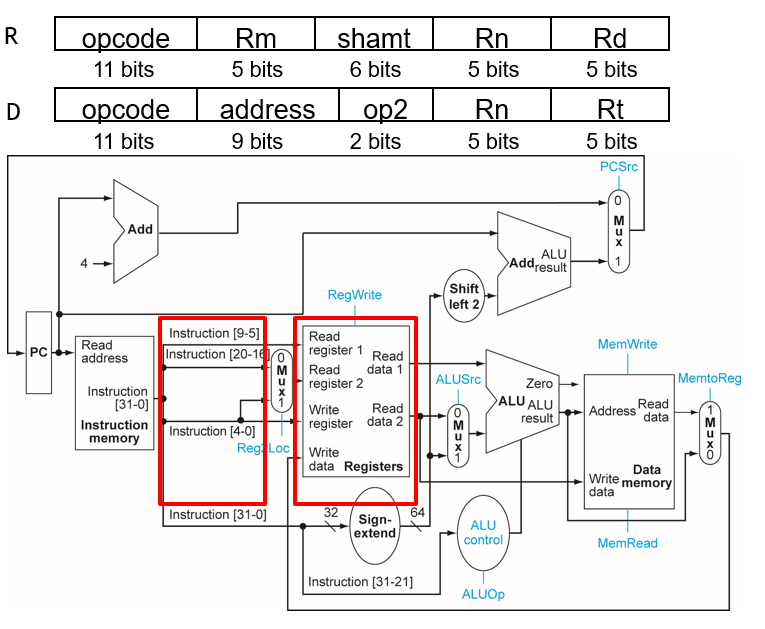
\includegraphics[width=4.75in]{../images/register_file_cutout.png}
	\end{center}
\end{figure} 


\clearpage
\section{Your Assignment}

You are to:
\begin{enumerate}
\item Create an instr\_parse module as described above.
\item Create and Expected Results Table for instr\_parse\_test.
\item Use the instr\_parse test module and verify that the instruction is being parsed properly by comparing to the Expected Results Table.
\item Create a regfile module.
\item Create a regfile\_test module.
\item Create an Expected Results Table for regfile\_test.
\item Verify that the values are being stored and retrieved from the regfile properly by comparing the results with the Expected Results Table.
\item Write a lab report according to the LabN format.
\end{enumerate} 